\documentclass[border=6pt]{standalone}
\usepackage{pgfplots}
\pgfplotsset{compat=1.18}
\begin{document}
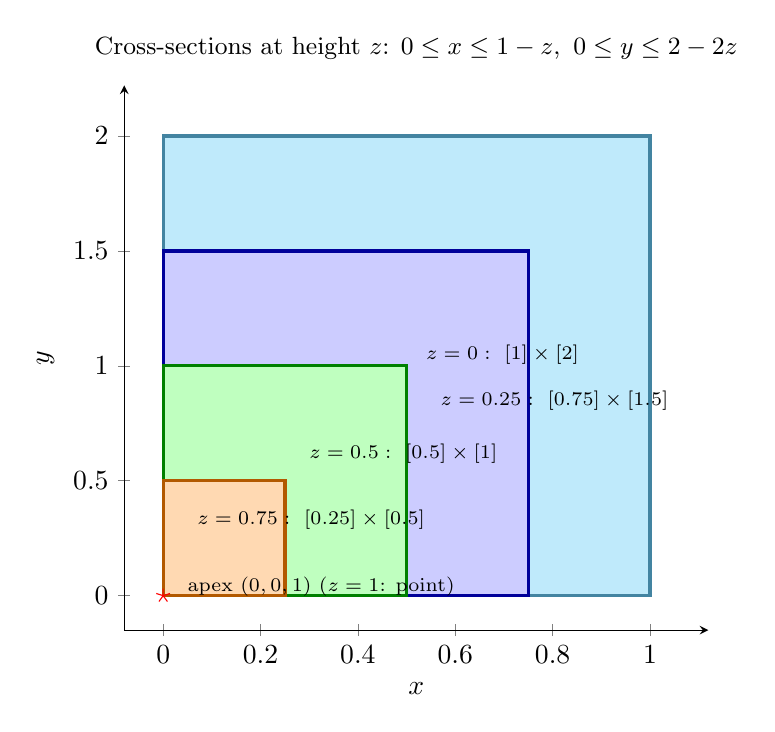
\begin{tikzpicture}
\begin{axis}[
    width=9cm, height=8.5cm,
    xlabel=$x$, ylabel=$y$,
    xmin=-0.08, xmax=1.12, ymin=-0.15, ymax=2.22,
    axis lines=left, grid=none,
    title={\small Cross-sections at height $z$: $0\le x\le 1-z,\ 0\le y\le 2-2z$},
]
% guide lines
\addplot[dashed, gray, forget plot] coordinates {(0,0) (0,2)};
\addplot[dashed, gray, forget plot] coordinates {(0,0) (1,0)};
% --- fills (drawn first) ---
\addplot[fill=cyan!25, draw=cyan!60!black, very thick, forget plot]
  coordinates {(0,0) (1,0) (1,2) (0,2)} -- cycle;
\addplot[fill=blue!20, draw=blue!60!black, very thick, forget plot]
  coordinates {(0,0) (0.75,0) (0.75,1.5) (0,1.5)} -- cycle;
\addplot[fill=green!25, draw=green!50!black, very thick, forget plot]
  coordinates {(0,0) (0.5,0) (0.5,1.0) (0,1.0)} -- cycle;
\addplot[fill=orange!30, draw=orange!70!black, very thick, forget plot]
  coordinates {(0,0) (0.25,0) (0.25,0.5) (0,0.5)} -- cycle;
% --- labels last so they stay on top ---
\node[anchor=west] at (axis cs:0.52,1.05) {\scriptsize $z=0:\ [1]\times[2]$};
\node[anchor=west] at (axis cs:0.55,0.85) {\scriptsize $z=0.25:\ [0.75]\times[1.5]$};
\node[anchor=west] at (axis cs:0.28,0.62) {\scriptsize $z=0.5:\ [0.5]\times[1]$};
\node[anchor=west] at (axis cs:0.05,0.33) {\scriptsize $z=0.75:\ [0.25]\times[0.5]$};
\addplot[only marks, mark=star, mark size=2.6pt, color=red] coordinates {(0,0)};
\node[anchor=west] at (axis cs:0.03,0.04) {\scriptsize apex $(0,0,1)$ ($z=1$: point)};
\end{axis}
\end{tikzpicture}
\end{document}
